\documentclass[aspectratio=169,10pt]{beamer}

\usetheme{Madrid}
\usecolortheme{default}
\setbeamertemplate{navigation symbols}{}
\setbeamertemplate{footline}[frame number]

\usepackage{amsmath,amssymb,booktabs,mathtools}
\usepackage{hyperref}
\usepackage{tikz}
\usetikzlibrary{arrows.meta,positioning,decorations.pathreplacing,shapes.geometric}
\usepackage{graphicx}
\usepackage{multicol}

% Semantic colors
\definecolor{positive}{HTML}{0173B2}
\definecolor{negative}{HTML}{DE8F05}
\definecolor{emphasis}{HTML}{029E73}
\definecolor{neutral}{gray}{0.55}
\definecolor{cbPurple}{HTML}{CC78BC}
\definecolor{lightbg}{HTML}{F0F4F8}
\newcommand{\pos}[1]{\textcolor{positive}{#1}}
\renewcommand{\neg}[1]{\textcolor{negative}{#1}}
\newcommand{\HL}[1]{\textcolor{emphasis}{#1}}

\title{Clinical Outcomes of Endoscopic Papillectomy\\for Ampullary Adenoma and Adenocarcinoma}
\subtitle{A Multicenter Retrospective Study in Japan}
\author{Presenter: [name]}
\institute{Shanghai Jiao Tong University}
\date{March 2026}

\begin{document}

% ============================================================
% SLIDE 1: Title
% ============================================================
\begin{frame}
\titlepage
\vspace{-10pt}
{\small Iwasaki E, et al. \textit{Gastrointestinal Endoscopy}. 2025.}
\end{frame}

% ============================================================
% SLIDE 2: Ampullary Anatomy and Tumors
% ============================================================
\begin{frame}{Ampulla of Vater: Anatomy and Tumor Overview}
\begin{columns}[T]
\column{0.48\textwidth}
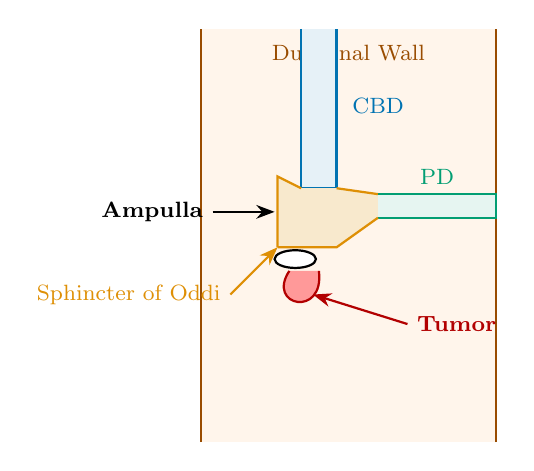
\begin{tikzpicture}[scale=0.75, every node/.style={font=\small}]
  % Duodenum wall
  \fill[orange!8] (-0.5,-3.5) rectangle (4.5,3.5);
  \draw[thick, orange!60!black] (-0.5,-3.5) -- (-0.5,3.5);
  \draw[thick, orange!60!black] (4.5,-3.5) -- (4.5,3.5);
  \node[font=\footnotesize, orange!60!black] at (2,3.1) {Duodenal Wall};

  % Common bile duct
  \draw[thick, positive, fill=positive!10] (1.2,3.5) -- (1.2,0.8) -- (1.8,0.8) -- (1.8,3.5);
  \node[font=\footnotesize, positive, right] at (1.9,2.2) {CBD};

  % Pancreatic duct
  \draw[thick, emphasis, fill=emphasis!10] (2.5,0.3) -- (4.5,0.3) -- (4.5,0.7) -- (2.5,0.7);
  \node[font=\footnotesize, emphasis, above] at (3.5,0.7) {PD};

  % Ampulla region
  \fill[negative!20] (0.8,-0.2) -- (0.8,1.0) -- (1.2,0.8)
    -- (1.8,0.8) -- (2.5,0.7) -- (2.5,0.3)
    -- (1.8,-0.2) -- cycle;
  \draw[thick, negative] (0.8,-0.2) -- (0.8,1.0) -- (1.2,0.8);
  \draw[thick, negative] (1.8,0.8) -- (2.5,0.7);
  \draw[thick, negative] (2.5,0.3) -- (1.8,-0.2) -- (0.8,-0.2);

  % Sphincter of Oddi label
  \draw[thick, negative, -{Stealth}] (0.0,-1.0) -- (0.8,-0.2);
  \node[font=\footnotesize, negative, left] at (0.0,-1.0) {Sphincter of Oddi};

  % Papilla opening
  \fill[white] (1.1,-0.4) ellipse (0.35 and 0.15);
  \draw[thick] (1.1,-0.4) ellipse (0.35 and 0.15);

  % Ampulla label
  \draw[-{Stealth}, thick] (-0.3,0.4) -- (0.75,0.4);
  \node[font=\footnotesize\bfseries, left] at (-0.3,0.4) {Ampulla};

  % Tumor illustration
  \fill[red!40] (1.0,-0.6) .. controls (0.6,-1.2) and (1.6,-1.4) .. (1.5,-0.6);
  \draw[thick, red!70!black] (1.0,-0.6) .. controls (0.6,-1.2) and (1.6,-1.4) .. (1.5,-0.6);
  \draw[-{Stealth}, thick, red!70!black] (3.0,-1.5) -- (1.4,-1.0);
  \node[font=\footnotesize\bfseries, red!70!black, right] at (3.0,-1.5) {Tumor};
\end{tikzpicture}

\column{0.48\textwidth}
\textbf{Ampullary epithelial tumors}
\begin{itemize}
  \item Rare tumors at the junction of CBD, PD, and duodenum
  \item Predominantly \textbf{adenomas} and \textbf{adenocarcinomas}
  \item Adenoma--carcinoma sequence applies
  \item Detection $\uparrow$ with routine upper endoscopy
\end{itemize}

\vspace{6pt}
\textbf{Why does anatomy matter?}
\begin{itemize}
  \item Complex 3-duct convergence $\to$ difficult margin assessment
  \item Sphincter of Oddi involvement affects staging
\end{itemize}
\end{columns}
\end{frame}

% ============================================================
% SLIDE 3: EP Technique and Indications
% ============================================================
\begin{frame}{Endoscopic Papillectomy: Technique and Indications}
\begin{columns}[T]
\column{0.55\textwidth}
\textbf{EP vs. Pancreaticoduodenectomy (PD)}
\begin{itemize}
  \item PD: historically standard, but high morbidity (30--50\%)
  \item \pos{EP}: minimally invasive, organ-preserving
  \item Guidelines recommend EP as \textbf{first-line} for ampullary adenomas without intraductal invasion
\end{itemize}

\vspace{6pt}
\textbf{Key procedural steps}
\begin{itemize}
  \item Duodenoscope + snare polypectomy
  \item Submucosal injection if laterally spreading
  \item Prophylactic PD/BD stenting (93.6\% / 82.5\%)
  \item APC for suspected residual lesion
  \item Clip closure of mucosal defect
\end{itemize}

\column{0.40\textwidth}
\begin{alertblock}{Guideline Recommendations}
  \begin{itemize}
    \item ESGE 2021
    \item JGES 2022
    \item ASGE 2015
  \end{itemize}
  EP = first-line for ampullary adenoma without intraductal extension
\end{alertblock}

\vspace{6pt}
\textbf{Clinical challenge}\\
Pre-EP biopsy accuracy is \neg{limited} $\to$ adenocarcinoma often found \emph{after} EP
\end{columns}
\end{frame}

% ============================================================
% SLIDE 4: Research Gap and Objectives
% ============================================================
\begin{frame}{Research Gap and Study Objectives}
\textbf{What we know}
\begin{itemize}
  \item EP is effective and safe for ampullary adenomas
  \item Reported recurrence rates: 0\%--33\% (wide variation)
\end{itemize}

\vspace{4pt}
\textbf{What we don't know}
\begin{itemize}
  \item \neg{Lack of large-scale, multicenter data} on long-term recurrence
  \item Predictors of recurrence remain poorly defined
  \item Role of pathologic margin status (R0/R1/Rx) unclear
\end{itemize}

\vspace{4pt}
\begin{exampleblock}{Study Objectives}
\begin{enumerate}
  \item Evaluate \textbf{cumulative recurrence rates} after EP in a nationwide cohort
  \item Identify \textbf{independent predictors} of recurrence
  \item Analyze recurrence in the \textbf{R0 resection subgroup}
\end{enumerate}
\end{exampleblock}
\end{frame}

% ============================================================
% SLIDE 5: Study Design
% ============================================================
\begin{frame}{Study Design}
\begin{columns}[T]
\column{0.55\textwidth}
\begin{itemize}
  \item \textbf{Design}: multicenter retrospective cohort
  \item \textbf{Setting}: 22 tertiary centers across Japan
  \item \textbf{Period}: January 2009 -- December 2020
  \item \textbf{Registry}: centralized web-based (UMIN)
  \item \textbf{Ethics}: opt-out, IRB-approved at each center
\end{itemize}

\vspace{4pt}
\textbf{Inclusion}: all patients undergoing EP\\
\textbf{Exclusion}:
\begin{itemize}
  \item Non-epithelial tumors on post-EP pathology
  \item Surgery for confirmed/suspected residual carcinoma
  \item EP-related mortality
\end{itemize}

\column{0.40\textwidth}
\textbf{Outcome definitions}
\begin{itemize}
  \item \textbf{Primary}: cumulative recurrence (histologically confirmed)
  \item \textbf{Secondary}: adverse events, retreatment success
\end{itemize}

\vspace{4pt}
\textbf{Statistical methods}
\begin{itemize}
  \item Kaplan--Meier + log-rank test
  \item Cox proportional hazards (multivariable)
  \item Censored at 5 years
\end{itemize}
\end{columns}
\end{frame}

% ============================================================
% SLIDE 6: Patient Flowchart
% ============================================================
\begin{frame}{Patient Flowchart}
\begin{center}
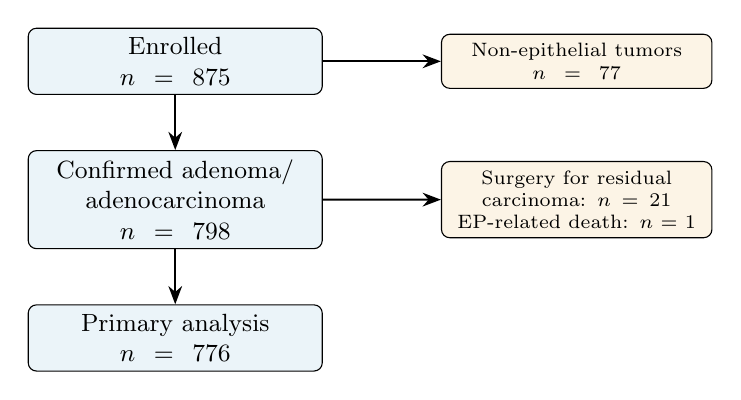
\begin{tikzpicture}[
  box/.style={draw, rounded corners=3pt, minimum width=3.2cm, minimum height=0.7cm,
              font=\small, fill=positive!8, text width=3.5cm, align=center},
  excl/.style={draw, rounded corners=3pt, minimum width=2.4cm, minimum height=0.55cm,
               font=\scriptsize, fill=negative!10, text width=3.2cm, align=center},
  arr/.style={-{Stealth}, thick},
  scale=0.9
]
  \node[box] (A) {Enrolled\\$n = 875$};
  \node[box, below=0.7cm of A] (B) {Confirmed adenoma/\\adenocarcinoma\\$n = 798$};
  \node[box, below=0.7cm of B] (C) {Primary analysis\\$n = 776$};

  \node[excl, right=1.5cm of A] (E1) {Non-epithelial tumors\\$n = 77$};
  \node[excl, right=1.5cm of B] (E2) {Surgery for residual\\carcinoma: $n=21$\\EP-related death: $n=1$};

  \draw[arr] (A) -- (B);
  \draw[arr] (B) -- (C);
  \draw[arr] (A) -- (E1);
  \draw[arr] (B) -- (E2);
\end{tikzpicture}
\end{center}

\vspace{2pt}
Median follow-up: \textbf{33 months} (IQR 6.75--60)
\end{frame}

% ============================================================
% SLIDE 7: R Classification and Definitions
% ============================================================
\begin{frame}{Pathologic Resection Status: R Classification}
\begin{columns}[T]
\column{0.55\textwidth}
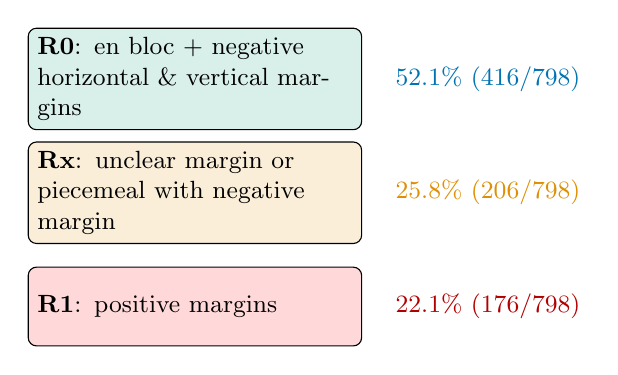
\begin{tikzpicture}[
  rbox/.style={draw, rounded corners=3pt, minimum width=3.8cm, minimum height=1.0cm,
               font=\small, text width=4.0cm, align=left},
  scale=0.85
]
  \node[rbox, fill=emphasis!15] (R0) at (0,2.5) {
    \textbf{R0}: en bloc + negative\\horizontal \& vertical margins
  };
  \node[rbox, fill=negative!15] (Rx) at (0,0.8) {
    \textbf{Rx}: unclear margin or\\piecemeal with negative margin
  };
  \node[rbox, fill=red!15] (R1) at (0,-0.9) {
    \textbf{R1}: positive margins
  };

  \node[font=\small, right=0.3cm of R0, positive] {52.1\% (416/798)};
  \node[font=\small, right=0.3cm of Rx, negative] {25.8\% (206/798)};
  \node[font=\small, right=0.3cm of R1, red!70!black] {22.1\% (176/798)};
\end{tikzpicture}

\column{0.40\textwidth}
\textbf{Key points}
\begin{itemize}
  \item Among en bloc resections, only \neg{58.6\%} achieved R0
  \item Thermal artifact $\to$ margin assessment difficulty
  \item En bloc $\neq$ R0 in ampullary EP
\end{itemize}

\vspace{4pt}
\textbf{Recurrence definition}\\
Histologic confirmation of neoplastic tissue during surveillance (every 6--12 months)
\end{columns}
\end{frame}

% ============================================================
% SLIDE 8: Baseline Characteristics
% ============================================================
\begin{frame}{Baseline Characteristics ($n = 798$)}
\begin{center}
\small
\begin{tabular}{@{}lrl@{}}
\toprule
\textbf{Variable} & \textbf{Value} & \\
\midrule
Age, median (IQR) & 67 (58--73) & years \\
Female & 320 & (40.1\%) \\
FAP & 53 & (6.6\%) \\
Tumor size, median (IQR) & 15 (10--20) & mm \\
LST-p & 121 & (15.2\%) \\
\midrule
\textbf{Resection method} & & \\
\quad En bloc & 710 & (89.0\%) \\
\quad Piecemeal & 88 & (11.0\%) \\
Technical success & 757 & (94.9\%) \\
\midrule
\textbf{Final pathologic diagnosis} & & \\
\quad Adenoma & 618 & (77.4\%) \\
\quad Carcinoma in adenoma & 88 & (11.0\%) \\
\quad Adenocarcinoma & 92 & (11.5\%) \\
\midrule
Expert operator ($\geq$20 cases) & 509 & (63.8\%) \\
\bottomrule
\end{tabular}
\end{center}
\end{frame}

% ============================================================
% SLIDE 9: Overall Recurrence (KM curve)
% ============================================================
\begin{frame}{Primary Outcome: Cumulative Recurrence After EP}
\begin{columns}[T]
\column{0.55\textwidth}
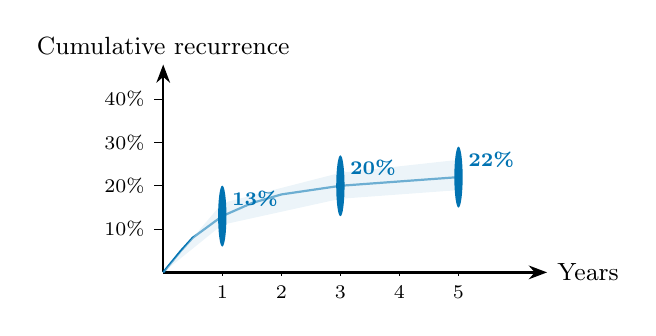
\begin{tikzpicture}[xscale=0.75, yscale=5.5]
  % Axes
  \draw[-{Stealth}, thick] (0,0) -- (6.5,0) node[right, font=\small] {Years};
  \draw[-{Stealth}, thick] (0,0) -- (0,0.48) node[above, font=\small] {Cumulative recurrence};

  % Y-axis ticks
  \foreach \y/\lab in {0.1/10\%, 0.2/20\%, 0.3/30\%, 0.4/40\%} {
    \draw (0,\y) -- (-0.15,\y) node[left, font=\scriptsize] {\lab};
  }
  % X-axis ticks
  \foreach \x/\lab in {1/1, 2/2, 3/3, 4/4, 5/5} {
    \draw (\x,0) -- (\x,-0.008) node[below, font=\scriptsize] {\lab};
  }

  % KM curve (overall)
  \draw[thick, positive] (0,0) -- (0.3,0.05) -- (0.5,0.08) -- (1,0.13)
    -- (1.5,0.16) -- (2,0.18) -- (3,0.20) -- (4,0.21) -- (5,0.22);

  % CI shading
  \fill[positive!15, opacity=0.5]
    (0,0) -- (1,0.11) -- (3,0.17) -- (5,0.19)
    -- (5,0.26) -- (3,0.23) -- (1,0.16) -- (0,0) -- cycle;

  % Key points
  \pgfmathsetmacro{\yOne}{0.13}
  \pgfmathsetmacro{\yThree}{0.20}
  \pgfmathsetmacro{\yFive}{0.22}
  \fill[positive] (1,\yOne) circle (2pt);
  \fill[positive] (3,\yThree) circle (2pt);
  \fill[positive] (5,\yFive) circle (2pt);

  \node[above right, font=\scriptsize\bfseries, positive] at (1,\yOne) {13\%};
  \node[above right, font=\scriptsize\bfseries, positive] at (3,\yThree) {20\%};
  \node[above right, font=\scriptsize\bfseries, positive] at (5,\yFive) {22\%};
\end{tikzpicture}

\column{0.42\textwidth}
\textbf{Recurrence: 142/776 (18.3\%)}
\begin{itemize}
  \item 97.9\% local recurrence
  \item 2.1\% metastatic (3 cases)
  \item Median time to recurrence: \textbf{6 months}
\end{itemize}

\vspace{4pt}
\begin{alertblock}{Cumulative Recurrence}
  \begin{tabular}{@{}ll@{}}
    1-year & 13\% (11--16\%) \\
    3-year & 20\% (17--23\%) \\
    5-year & 22\% (19--26\%) \\
  \end{tabular}
\end{alertblock}
\end{columns}
\end{frame}

% ============================================================
% SLIDE 10: Recurrence by R Status
% ============================================================
\begin{frame}{Recurrence Stratified by Resection Margin Status}
\begin{columns}[T]
\column{0.55\textwidth}
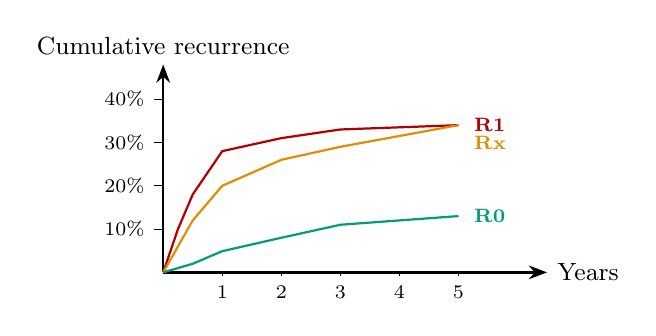
\begin{tikzpicture}[xscale=0.75, yscale=5.5]
  % Axes
  \draw[-{Stealth}, thick] (0,0) -- (6.5,0) node[right, font=\small] {Years};
  \draw[-{Stealth}, thick] (0,0) -- (0,0.48) node[above, font=\small] {Cumulative recurrence};

  % Y-axis ticks
  \foreach \y/\lab in {0.1/10\%, 0.2/20\%, 0.3/30\%, 0.4/40\%} {
    \draw (0,\y) -- (-0.15,\y) node[left, font=\scriptsize] {\lab};
  }
  % X-axis ticks
  \foreach \x/\lab in {1/1, 2/2, 3/3, 4/4, 5/5} {
    \draw (\x,0) -- (\x,-0.008) node[below, font=\scriptsize] {\lab};
  }

  % R1 curve (red)
  \draw[thick, red!70!black]
    (0,0) -- (0.25,0.10) -- (0.5,0.18) -- (1,0.28) -- (2,0.31) -- (3,0.33) -- (5,0.34);
  \node[right, font=\scriptsize\bfseries, red!70!black] at (5.1,0.34) {R1};

  % Rx curve (orange)
  \draw[thick, negative]
    (0,0) -- (0.25,0.06) -- (0.5,0.12) -- (1,0.20) -- (2,0.26) -- (3,0.29) -- (5,0.34);
  \node[right, font=\scriptsize\bfseries, negative] at (5.1,0.30) {Rx};

  % R0 curve (green)
  \draw[thick, emphasis]
    (0,0) -- (0.5,0.02) -- (1,0.049) -- (2,0.08) -- (3,0.11) -- (5,0.13);
  \node[right, font=\scriptsize\bfseries, emphasis] at (5.1,0.13) {R0};
\end{tikzpicture}

\column{0.42\textwidth}
\textbf{3-year cumulative recurrence}
\begin{itemize}
  \item \HL{R0}: \HL{11\%} (7.6--15\%)
  \item \neg{Rx}: \neg{29\%}
  \item \textcolor{red!70!black}{\textbf{R1}}: \textcolor{red!70!black}{\textbf{33\%}}
\end{itemize}

\vspace{3pt}
Log-rank $P < .001$

\vspace{4pt}
\textbf{Early recurrence ($\leq$6 months)}
\begin{itemize}
  \item R0: 3.0\% (12/415)
  \item Rx: 13.2\% (27/204)
  \item R1: 21.7\% (34/157)
\end{itemize}

\vspace{3pt}
\textbf{Median time to recurrence}\\
R0: 15 mo \quad Rx: 6 mo \quad R1: 3 mo
\end{columns}
\end{frame}

% ============================================================
% SLIDE 11: Cox Regression - Overall Cohort
% ============================================================
\begin{frame}{Multivariable Cox Regression: Overall Cohort}
\begin{center}
\small
\begin{tabular}{@{}lccc@{}}
\toprule
\textbf{Predictor} & \textbf{HR} & \textbf{95\% CI} & \textbf{$P$} \\
\midrule
Female & \textbf{1.48} & 1.06--2.08 & \pos{.022} \\
FAP & 1.59 & 0.90--2.83 & .11 \\
Large tumor ($\geq$15 mm) & 0.88 & 0.60--1.28 & .5 \\
LST-p & 1.39 & 0.91--2.12 & .13 \\
Piecemeal resection & \textbf{1.69} & 1.07--2.65 & \pos{.023} \\
Period 2015--2020 & \textbf{1.57} & 1.09--2.26 & \pos{.016} \\
APC use & 1.54 & 0.73--3.29 & .3 \\
\midrule
\multicolumn{4}{@{}l}{\textbf{Margin status} (ref: R0)} \\
\quad R1 (positive) & \textbf{2.95} & 1.87--4.66 & \pos{$<$.001} \\
\quad Rx (indeterminate) & \textbf{2.38} & 1.49--3.81 & \pos{$<$.001} \\
\midrule
\multicolumn{4}{@{}l}{\textbf{Final pathology} (ref: adenoma)} \\
\quad Carcinoma in adenoma & 1.07 & 0.60--1.91 & .8 \\
\quad Adenocarcinoma & \textbf{1.84} & 1.16--2.92 & \pos{.009} \\
\bottomrule
\end{tabular}
\end{center}

\vspace{2pt}
\HL{Margin status} = strongest predictor; \textbf{adenocarcinoma} independently associated with recurrence
\end{frame}

% ============================================================
% SLIDE 12: R0 Subgroup Analysis
% ============================================================
\begin{frame}{R0 Subgroup: Independent Predictors of Recurrence}
\begin{columns}[T]
\column{0.55\textwidth}
\small
\begin{tabular}{@{}lccc@{}}
\toprule
\textbf{Predictor} & \textbf{HR} & \textbf{95\% CI} & \textbf{$P$} \\
\midrule
Female & \textbf{2.09} & 1.07--4.07 & \pos{.032} \\
FAP & 2.90 & 0.95--8.89 & .063 \\
LST-p & 2.12 & 0.83--5.43 & .12 \\
APC use & \textbf{6.26} & 1.44--27.1 & \pos{.014} \\
BD invasion & \textbf{4.86} & 1.08--21.8 & \pos{.039} \\
Adenocarcinoma & \textbf{2.74} & 1.22--6.14 & \pos{.015} \\
\bottomrule
\end{tabular}

\vspace{6pt}
Even after R0 resection:\\
3-year cumulative recurrence = \neg{11\%}

\column{0.42\textwidth}
\begin{alertblock}{Why APC Is Significant?}
  APC used when residual disease suspected endoscopically $\to$ \textbf{marker} of residual risk, not cause
\end{alertblock}

\vspace{4pt}
\begin{exampleblock}{Why Bile Duct Invasion?}
  Ductal involvement $\to$ difficult margin assessment $\to$ microscopic residual disease despite ``R0''
\end{exampleblock}
\end{columns}
\end{frame}

% ============================================================
% SLIDE 13: Adverse Events
% ============================================================
\begin{frame}{Adverse Events ($n = 798$)}
\begin{columns}[T]
\column{0.50\textwidth}
\begin{center}
\small
\begin{tabular}{@{}lrr@{}}
\toprule
\textbf{Adverse Event} & \textbf{$n$ (\%)} & \textbf{Severe} \\
\midrule
\textbf{All AEs} & 259 (32.5) & 31 (3.9\%) \\
\midrule
Bleeding & 155 (19.4) & 10 (1.3\%) \\
Pancreatitis & 110 (13.8) & 14 (1.8\%) \\
Cholangitis & 16 (2.0) & 0 \\
Perforation (intra) & 17 (2.1) & 7 (0.9\%) \\
Perforation (delayed) & 9 (1.1) & 4 (0.5\%) \\
Delayed BD stenosis & 19 (2.4) & --- \\
Delayed PD stenosis & 20 (2.5) & --- \\
\midrule
\textbf{Mortality} & \multicolumn{2}{c}{1 (0.1\%)} \\
\bottomrule
\end{tabular}
\end{center}

\column{0.45\textwidth}
\textbf{Key observations}
\begin{itemize}
  \item \neg{Bleeding} most common (19.4\%), mostly mild
  \item \neg{Pancreatitis}: 13.8\%, severe in 1.8\%
  \item Overall severe AE rate: \textbf{3.9\%}
  \item 1 death: cirrhosis patient with delayed bleeding $\to$ liver failure
\end{itemize}

\vspace{4pt}
\textbf{Prophylactic measures}
\begin{itemize}
  \item PD stent: 93.6\%
  \item BD stent: 82.5\%
  \item Clip closure: 72.3\%
\end{itemize}
\end{columns}
\end{frame}

% ============================================================
% SLIDE 14: Retreatment Outcomes
% ============================================================
\begin{frame}{Retreatment for Local Recurrence}
\begin{columns}[T]
\column{0.50\textwidth}
\textbf{Local recurrence}: 139/142 (97.9\%)

\vspace{4pt}
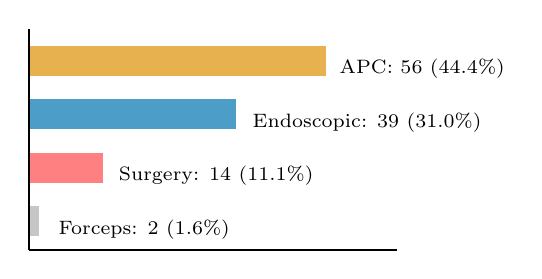
\begin{tikzpicture}[
  bar/.style={minimum height=0.45cm, anchor=west, font=\scriptsize},
  scale=0.85
]
  % APC
  \fill[negative!70] (0,3.0) rectangle (4.44,3.45);
  \node[bar] at (4.5,3.1) {APC: 56 (44.4\%)};

  % Endoscopic resection
  \fill[positive!70] (0,2.2) rectangle (3.10,2.65);
  \node[bar] at (3.2,2.3) {Endoscopic: 39 (31.0\%)};

  % Surgery
  \fill[red!50] (0,1.4) rectangle (1.11,1.85);
  \node[bar] at (1.2,1.5) {Surgery: 14 (11.1\%)};

  % Forceps
  \fill[neutral!50] (0,0.6) rectangle (0.16,1.05);
  \node[bar] at (0.3,0.7) {Forceps: 2 (1.6\%)};

  % Axis
  \draw[thick] (0,0.4) -- (0,3.7);
  \draw[thick] (0,0.4) -- (5.5,0.4);
\end{tikzpicture}

\column{0.45\textwidth}
\begin{exampleblock}{Endoscopic Retreatment Success}
  \textbf{74.5\%} (70/97) achieved clinical success\\[4pt]
  = no adenoma/carcinoma detected on follow-up biopsy
\end{exampleblock}

\vspace{6pt}
\textbf{Clinical implication}
\begin{itemize}
  \item Most recurrences manageable endoscopically
  \item Surgery needed in only \textbf{11.1\%} of recurrent cases
  \item Supports \pos{surveillance strategy} over upfront surgery
\end{itemize}
\end{columns}
\end{frame}

% ============================================================
% SLIDE 15: Key Findings Summary
% ============================================================
\begin{frame}{Discussion: Key Findings}
\begin{enumerate}
  \item \textbf{Recurrence is common, even after R0}\\
  Overall 3-year: 20\%; R0 3-year: 11\% $\to$ \neg{long-term surveillance is mandatory}

  \vspace{6pt}
  \item \textbf{Margin status is the strongest predictor}\\
  R1 (HR 2.95) and Rx (HR 2.38) vs R0\\
  Early recurrence ($\leq$6 mo): R0 3\% vs R1 22\% $\to$ R1/Rx may represent residual disease

  \vspace{6pt}
  \item \textbf{Other significant predictors}\\
  Female sex, piecemeal resection, adenocarcinoma, later treatment era (2015--2020)\\
  Later era: likely reflects influx of less experienced operators ($<$20 cases: 26\% $\to$ 44\%)
\end{enumerate}
\end{frame}

% ============================================================
% SLIDE 16: R0 Definition Refinement
% ============================================================
\begin{frame}{Rethinking the R0 Definition}
\begin{columns}[T]
\column{0.55\textwidth}
\textbf{Current R0 definition}\\
Negative horizontal + vertical margins by en bloc resection

\vspace{6pt}
\textbf{Problem}: 11\% recurrence after ``R0''

\vspace{4pt}
\textbf{Contributing factors}:
\begin{itemize}
  \item \neg{Bile duct invasion} (HR 4.86 in R0 subgroup)
  \item Anatomical complexity $\to$ margin assessment difficulty
  \item 17\% of R0 patients received APC (endoscopic suspicion of residual disease)
\end{itemize}

\column{0.42\textwidth}
\begin{alertblock}{Proposed Refinement}
  Incorporate \textbf{absence of ductal invasion} into R0 criteria to improve prognostic accuracy
\end{alertblock}

\vspace{6pt}
\textbf{Comparison with other GI tumors}
\begin{itemize}
  \item Ampullary EP R0: 11\% recurrence
  \item GI epithelial ESD R0: 5.8\%
  \item Gap likely due to anatomical complexity
\end{itemize}
\end{columns}
\end{frame}

% ============================================================
% SLIDE 17: Limitations
% ============================================================
\begin{frame}{Limitations}
\begin{enumerate}
  \item \textbf{Retrospective design} over 10-year span across 22 centers\\
  $\to$ potential missing data and selection bias

  \vspace{4pt}
  \item \textbf{Heterogeneity in practice}\\
  EP technique, surveillance intervals, APC use varied by institution and era\\
  (mitigated by stratification by treatment period)

  \vspace{4pt}
  \item \textbf{High-volume center bias}\\
  All 22 centers are tertiary referral $\to$ generalizability may be limited

  \vspace{4pt}
  \item \textbf{Local pathologic assessment}\\
  No central pathology review $\to$ inter-observer variability

  \vspace{4pt}
  \item \textbf{No T1a/T1b differentiation}\\
  Adenocarcinoma not substaged $\to$ cannot assess depth-specific recurrence risk
\end{enumerate}
\end{frame}

% ============================================================
% SLIDE 18: Take-home Messages
% ============================================================
\begin{frame}{Take-Home Messages}
\begin{enumerate}
  \item[\HL{1.}] \textbf{Recurrence after EP is not rare}\\
  20\% at 3 years overall; 11\% even in R0 $\to$
  \HL{long-term endoscopic surveillance is essential for ALL patients}

  \vspace{8pt}
  \item[\HL{2.}] \textbf{Pursue R0 resection, but understand its limits}\\
  R0 dramatically reduces recurrence vs R1/Rx, but does not eliminate it\\
  $\to$ \HL{bile duct invasion and adenocarcinoma remain risks even in R0}

  \vspace{8pt}
  \item[\HL{3.}] \textbf{Recurrence is manageable}\\
  97.9\% local, 74.5\% endoscopic retreatment success\\
  $\to$ \HL{EP + surveillance is a viable long-term strategy}
\end{enumerate}
\end{frame}

% ============================================================
% SLIDE 19: References
% ============================================================
\begin{frame}{References}
\small
\begin{thebibliography}{9}
  \bibitem{iwasaki2025} Iwasaki E, et al. Clinical outcomes of endoscopic papillectomy for ampullary adenoma and adenocarcinoma: a multicenter retrospective study in Japan. \textit{Gastrointest Endosc}. 2025.
  \bibitem{esge2021} Vanbiervliet G, et al. Endoscopic management of ampullary tumors: ESGE guideline. \textit{Endoscopy}. 2021;53:429--448.
  \bibitem{jges2022} Itoi T, et al. Clinical practice guidelines for endoscopic papillectomy. \textit{Dig Endosc}. 2022;34:394--411.
  \bibitem{kawashima2021} Kawashima H, et al. Endoscopic papillectomy for ampullary adenoma and early adenocarcinoma. \textit{Dig Endosc}. 2021;33:858--869.
  \bibitem{hollenbach2025} Hollenbach M, et al. Endoscopic papillectomy versus surgical ampullectomy for adenomas and early cancers of the papilla. \textit{Gut}. 2025;74:397--409.
  \bibitem{singh2024} Singh AD, et al. Incidence and risk factors for recurrence of ampullary adenomas after endoscopic papillectomy. \textit{Dig Endosc}. 2024;36:834--842.
\end{thebibliography}
\end{frame}

% ============================================================
% SLIDE 20: Thank You
% ============================================================
\begin{frame}
\centering
\vspace{1.5cm}
{\Large\bfseries Thank You}\\[12pt]
{\large Questions \& Discussion}\\[20pt]
\textcolor{neutral}{\small Presenter: [name] $\mid$ Shanghai Jiao Tong University}
\end{frame}

% ============================================================
% BACKUP SLIDES
% ============================================================
\appendix
\begin{frame}{Backup Slides}
\centering
{\large\textcolor{neutral}{Additional materials for Q\&A}}
\end{frame}

% BACKUP 1: Recurrence by Pathologic Diagnosis
\begin{frame}{Backup: Recurrence by Final Pathologic Diagnosis}
\textbf{3-year cumulative recurrence by histology}
\begin{itemize}
  \item Adenoma: 19\% (95\% CI, 15--22\%)
  \item Carcinoma in adenoma: 20\% (16--24\%)
  \item Adenocarcinoma: 25\% (20--30\%)
\end{itemize}
Log-rank $P < .001$

\vspace{6pt}
\textbf{Interpretation}
\begin{itemize}
  \item Carcinoma-in-adenoma recurs at similar rate to adenoma
  \item Adenocarcinoma carries \neg{highest recurrence risk}
  \item Limitation: T1a vs T1b not differentiated
\end{itemize}
\end{frame}

% BACKUP 2: Detailed AE Table
\begin{frame}{Backup: Detailed Adverse Event Severity}
\begin{center}
\small
\begin{tabular}{@{}lcccc@{}}
\toprule
\textbf{AE} & \textbf{Mild} & \textbf{Moderate} & \textbf{Severe} & \textbf{Total} \\
\midrule
Pancreatitis & 63 (7.9\%) & 33 (4.1\%) & 14 (1.8\%) & 110 (13.8\%) \\
Bleeding & 125 (15.7\%) & 20 (2.5\%) & 10 (1.3\%) & 155 (19.4\%) \\
Cholangitis & 7 (0.9\%) & 9 (1.1\%) & 0 & 16 (2.0\%) \\
Perforation (intra) & 7 (0.9\%) & 3 (0.4\%) & 7 (0.9\%) & 17 (2.1\%) \\
Perforation (delayed) & 3 (0.4\%) & 2 (0.3\%) & 4 (0.5\%) & 9 (1.1\%) \\
\midrule
Mortality & \multicolumn{4}{c}{1 (0.1\%)} \\
\bottomrule
\end{tabular}
\end{center}

\vspace{6pt}
Severity graded by ASGE classification (Cotton et al. 2010)
\end{frame}

% BACKUP 3: EP Procedure Details
\begin{frame}{Backup: EP Procedural Details}
\begin{columns}[T]
\column{0.48\textwidth}
\textbf{Electrocautery mode}
\begin{itemize}
  \item Mixed current: 55.5\%
  \item Pure cutting: 44.5\%
\end{itemize}

\vspace{4pt}
\textbf{Prophylactic measures}
\begin{itemize}
  \item PD stent: 93.6\%
  \item PD sphincterotomy: 7.9\%
  \item BD stent: 82.5\%
  \item Biliary sphincterotomy: 16.0\%
\end{itemize}

\column{0.48\textwidth}
\textbf{Clip closure}
\begin{itemize}
  \item Partial ($<$50\%): 49.5\%
  \item Sufficient ($\geq$50\%): 22.8\%
  \item None: 27.7\%
\end{itemize}

\vspace{4pt}
\textbf{Pre-resection evaluation}
\begin{itemize}
  \item EUS: 81.5\% (650/798)
  \item Other imaging: 132
  \item None: 18
\end{itemize}
\end{columns}
\end{frame}

\end{document}
